\documentclass[letterpaper]{article} % DO NOT CHANGE THIS
\usepackage[submission]{aaai2026}  % DO NOT CHANGE THIS
\usepackage{times}  % DO NOT CHANGE THIS
\usepackage{helvet}  % DO NOT CHANGE THIS
\usepackage{courier}  % DO NOT CHANGE THIS
\usepackage[hyphens]{url}  % DO NOT CHANGE THIS
\usepackage{graphicx} % DO NOT CHANGE THIS
\urlstyle{rm} % DO NOT CHANGE THIS
\def\UrlFont{\rm}  % DO NOT CHANGE THIS
\usepackage{natbib}  % DO NOT CHANGE THIS AND DO NOT ADD ANY OPTIONS TO IT
\usepackage{caption} % DO NOT CHANGE THIS AND DO NOT ADD ANY OPTIONS TO IT
\frenchspacing  % DO NOT CHANGE THIS
\setlength{\pdfpagewidth}{8.5in} % DO NOT CHANGE THIS
\setlength{\pdfpageheight}{11in} % DO NOT CHANGE THIS
%
% These are recommended to typeset algorithms but not required. See the subsubsection on algorithms. Remove them if you don't have algorithms in your paper.
\usepackage{algorithm}
\usepackage{algorithmic}
\pagestyle{plain}
\usepackage{threeparttable}
%%%%% NEW MATH DEFINITIONS %%%%%

\usepackage{amsmath,amsfonts,bm}

% Mark sections of captions for referring to divisions of figures
\newcommand{\figleft}{{\em (Left)}}
\newcommand{\figcenter}{{\em (Center)}}
\newcommand{\figright}{{\em (Right)}}
\newcommand{\figtop}{{\em (Top)}}
\newcommand{\figbottom}{{\em (Bottom)}}
\newcommand{\captiona}{{\em (a)}}
\newcommand{\captionb}{{\em (b)}}
\newcommand{\captionc}{{\em (c)}}
\newcommand{\captiond}{{\em (d)}}

% Highlight a newly defined term
\newcommand{\newterm}[1]{{\bf #1}}


% Figure reference, lower-case.
\def\figref#1{figure~\ref{#1}}
% Figure reference, capital. For start of sentence
\def\Figref#1{Figure~\ref{#1}}
\def\twofigref#1#2{figures \ref{#1} and \ref{#2}}
\def\quadfigref#1#2#3#4{figures \ref{#1}, \ref{#2}, \ref{#3} and \ref{#4}}
% Section reference, lower-case.
\def\secref#1{section~\ref{#1}}
% Section reference, capital.
\def\Secref#1{Section~\ref{#1}}
% Reference to two sections.
\def\twosecrefs#1#2{sections \ref{#1} and \ref{#2}}
% Reference to three sections.
\def\secrefs#1#2#3{sections \ref{#1}, \ref{#2} and \ref{#3}}
% Reference to an equation, lower-case.
\def\eqref#1{equation~\ref{#1}}
% Reference to an equation, upper case
\def\Eqref#1{Equation~\ref{#1}}
% A raw reference to an equation---avoid using if possible
\def\plaineqref#1{\ref{#1}}
% Reference to a chapter, lower-case.
\def\chapref#1{chapter~\ref{#1}}
% Reference to an equation, upper case.
\def\Chapref#1{Chapter~\ref{#1}}
% Reference to a range of chapters
\def\rangechapref#1#2{chapters\ref{#1}--\ref{#2}}
% Reference to an algorithm, lower-case.
\def\algref#1{algorithm~\ref{#1}}
% Reference to an algorithm, upper case.
\def\Algref#1{Algorithm~\ref{#1}}
\def\twoalgref#1#2{algorithms \ref{#1} and \ref{#2}}
\def\Twoalgref#1#2{Algorithms \ref{#1} and \ref{#2}}
% Reference to a part, lower case
\def\partref#1{part~\ref{#1}}
% Reference to a part, upper case
\def\Partref#1{Part~\ref{#1}}
\def\twopartref#1#2{parts \ref{#1} and \ref{#2}}

\def\ceil#1{\lceil #1 \rceil}
\def\floor#1{\lfloor #1 \rfloor}
\def\1{\bm{1}}
\newcommand{\train}{\mathcal{D}}
\newcommand{\valid}{\mathcal{D_{\mathrm{valid}}}}
\newcommand{\test}{\mathcal{D_{\mathrm{test}}}}

\def\eps{{\epsilon}}


% Random variables
\def\reta{{\textnormal{$\eta$}}}
\def\ra{{\textnormal{a}}}
\def\rb{{\textnormal{b}}}
\def\rc{{\textnormal{c}}}
\def\rd{{\textnormal{d}}}
\def\re{{\textnormal{e}}}
\def\rf{{\textnormal{f}}}
\def\rg{{\textnormal{g}}}
\def\rh{{\textnormal{h}}}
\def\ri{{\textnormal{i}}}
\def\rj{{\textnormal{j}}}
\def\rk{{\textnormal{k}}}
\def\rl{{\textnormal{l}}}
% rm is already a command, just don't name any random variables m
\def\rn{{\textnormal{n}}}
\def\ro{{\textnormal{o}}}
\def\rp{{\textnormal{p}}}
\def\rq{{\textnormal{q}}}
\def\rr{{\textnormal{r}}}
\def\rs{{\textnormal{s}}}
\def\rt{{\textnormal{t}}}
\def\ru{{\textnormal{u}}}
\def\rv{{\textnormal{v}}}
\def\rw{{\textnormal{w}}}
\def\rx{{\textnormal{x}}}
\def\ry{{\textnormal{y}}}
\def\rz{{\textnormal{z}}}

% Random vectors
\def\rvepsilon{{\mathbf{\epsilon}}}
\def\rvtheta{{\mathbf{\theta}}}
\def\rva{{\mathbf{a}}}
\def\rvb{{\mathbf{b}}}
\def\rvc{{\mathbf{c}}}
\def\rvd{{\mathbf{d}}}
\def\rve{{\mathbf{e}}}
\def\rvf{{\mathbf{f}}}
\def\rvg{{\mathbf{g}}}
\def\rvh{{\mathbf{h}}}
\def\rvu{{\mathbf{i}}}
\def\rvj{{\mathbf{j}}}
\def\rvk{{\mathbf{k}}}
\def\rvl{{\mathbf{l}}}
\def\rvm{{\mathbf{m}}}
\def\rvn{{\mathbf{n}}}
\def\rvo{{\mathbf{o}}}
\def\rvp{{\mathbf{p}}}
\def\rvq{{\mathbf{q}}}
\def\rvr{{\mathbf{r}}}
\def\rvs{{\mathbf{s}}}
\def\rvt{{\mathbf{t}}}
\def\rvu{{\mathbf{u}}}
\def\rvv{{\mathbf{v}}}
\def\rvw{{\mathbf{w}}}
\def\rvx{{\mathbf{x}}}
\def\rvy{{\mathbf{y}}}
\def\rvz{{\mathbf{z}}}

% Elements of random vectors
\def\erva{{\textnormal{a}}}
\def\ervb{{\textnormal{b}}}
\def\ervc{{\textnormal{c}}}
\def\ervd{{\textnormal{d}}}
\def\erve{{\textnormal{e}}}
\def\ervf{{\textnormal{f}}}
\def\ervg{{\textnormal{g}}}
\def\ervh{{\textnormal{h}}}
\def\ervi{{\textnormal{i}}}
\def\ervj{{\textnormal{j}}}
\def\ervk{{\textnormal{k}}}
\def\ervl{{\textnormal{l}}}
\def\ervm{{\textnormal{m}}}
\def\ervn{{\textnormal{n}}}
\def\ervo{{\textnormal{o}}}
\def\ervp{{\textnormal{p}}}
\def\ervq{{\textnormal{q}}}
\def\ervr{{\textnormal{r}}}
\def\ervs{{\textnormal{s}}}
\def\ervt{{\textnormal{t}}}
\def\ervu{{\textnormal{u}}}
\def\ervv{{\textnormal{v}}}
\def\ervw{{\textnormal{w}}}
\def\ervx{{\textnormal{x}}}
\def\ervy{{\textnormal{y}}}
\def\ervz{{\textnormal{z}}}

% Random matrices
\def\rmA{{\mathbf{A}}}
\def\rmB{{\mathbf{B}}}
\def\rmC{{\mathbf{C}}}
\def\rmD{{\mathbf{D}}}
\def\rmE{{\mathbf{E}}}
\def\rmF{{\mathbf{F}}}
\def\rmG{{\mathbf{G}}}
\def\rmH{{\mathbf{H}}}
\def\rmI{{\mathbf{I}}}
\def\rmJ{{\mathbf{J}}}
\def\rmK{{\mathbf{K}}}
\def\rmL{{\mathbf{L}}}
\def\rmM{{\mathbf{M}}}
\def\rmN{{\mathbf{N}}}
\def\rmO{{\mathbf{O}}}
\def\rmP{{\mathbf{P}}}
\def\rmQ{{\mathbf{Q}}}
\def\rmR{{\mathbf{R}}}
\def\rmS{{\mathbf{S}}}
\def\rmT{{\mathbf{T}}}
\def\rmU{{\mathbf{U}}}
\def\rmV{{\mathbf{V}}}
\def\rmW{{\mathbf{W}}}
\def\rmX{{\mathbf{X}}}
\def\rmY{{\mathbf{Y}}}
\def\rmZ{{\mathbf{Z}}}

% Elements of random matrices
\def\ermA{{\textnormal{A}}}
\def\ermB{{\textnormal{B}}}
\def\ermC{{\textnormal{C}}}
\def\ermD{{\textnormal{D}}}
\def\ermE{{\textnormal{E}}}
\def\ermF{{\textnormal{F}}}
\def\ermG{{\textnormal{G}}}
\def\ermH{{\textnormal{H}}}
\def\ermI{{\textnormal{I}}}
\def\ermJ{{\textnormal{J}}}
\def\ermK{{\textnormal{K}}}
\def\ermL{{\textnormal{L}}}
\def\ermM{{\textnormal{M}}}
\def\ermN{{\textnormal{N}}}
\def\ermO{{\textnormal{O}}}
\def\ermP{{\textnormal{P}}}
\def\ermQ{{\textnormal{Q}}}
\def\ermR{{\textnormal{R}}}
\def\ermS{{\textnormal{S}}}
\def\ermT{{\textnormal{T}}}
\def\ermU{{\textnormal{U}}}
\def\ermV{{\textnormal{V}}}
\def\ermW{{\textnormal{W}}}
\def\ermX{{\textnormal{X}}}
\def\ermY{{\textnormal{Y}}}
\def\ermZ{{\textnormal{Z}}}

% Vectors
\def\vzero{{\bm{0}}}
\def\vone{{\bm{1}}}
\def\vmu{{\bm{\mu}}}
\def\vtheta{{\bm{\theta}}}
\def\va{{\bm{a}}}
\def\vb{{\bm{b}}}
\def\vc{{\bm{c}}}
\def\vd{{\bm{d}}}
\def\ve{{\bm{e}}}
\def\vf{{\bm{f}}}
\def\vg{{\bm{g}}}
\def\vh{{\bm{h}}}
\def\vi{{\bm{i}}}
\def\vj{{\bm{j}}}
\def\vk{{\bm{k}}}
\def\vl{{\bm{l}}}
\def\vm{{\bm{m}}}
\def\vn{{\bm{n}}}
\def\vo{{\bm{o}}}
\def\vp{{\bm{p}}}
\def\vq{{\bm{q}}}
\def\vr{{\bm{r}}}
\def\vs{{\bm{s}}}
\def\vt{{\bm{t}}}
\def\vu{{\bm{u}}}
\def\vv{{\bm{v}}}
\def\vw{{\bm{w}}}
\def\vx{{\bm{x}}}
\def\vy{{\bm{y}}}
\def\vz{{\bm{z}}}

% Elements of vectors
\def\evalpha{{\alpha}}
\def\evbeta{{\beta}}
\def\evepsilon{{\epsilon}}
\def\evlambda{{\lambda}}
\def\evomega{{\omega}}
\def\evmu{{\mu}}
\def\evpsi{{\psi}}
\def\evsigma{{\sigma}}
\def\evtheta{{\theta}}
\def\eva{{a}}
\def\evb{{b}}
\def\evc{{c}}
\def\evd{{d}}
\def\eve{{e}}
\def\evf{{f}}
\def\evg{{g}}
\def\evh{{h}}
\def\evi{{i}}
\def\evj{{j}}
\def\evk{{k}}
\def\evl{{l}}
\def\evm{{m}}
\def\evn{{n}}
\def\evo{{o}}
\def\evp{{p}}
\def\evq{{q}}
\def\evr{{r}}
\def\evs{{s}}
\def\evt{{t}}
\def\evu{{u}}
\def\evv{{v}}
\def\evw{{w}}
\def\evx{{x}}
\def\evy{{y}}
\def\evz{{z}}

% Matrix
\def\mA{{\bm{A}}}
\def\mB{{\bm{B}}}
\def\mC{{\bm{C}}}
\def\mD{{\bm{D}}}
\def\mE{{\bm{E}}}
\def\mF{{\bm{F}}}
\def\mG{{\bm{G}}}
\def\mH{{\bm{H}}}
\def\mI{{\bm{I}}}
\def\mJ{{\bm{J}}}
\def\mK{{\bm{K}}}
\def\mL{{\bm{L}}}
\def\mM{{\bm{M}}}
\def\mN{{\bm{N}}}
\def\mO{{\bm{O}}}
\def\mP{{\bm{P}}}
\def\mQ{{\bm{Q}}}
\def\mR{{\bm{R}}}
\def\mS{{\bm{S}}}
\def\mT{{\bm{T}}}
\def\mU{{\bm{U}}}
\def\mV{{\bm{V}}}
\def\mW{{\bm{W}}}
\def\mX{{\bm{X}}}
\def\mY{{\bm{Y}}}
\def\mZ{{\bm{Z}}}
\def\mBeta{{\bm{\beta}}}
\def\mPhi{{\bm{\Phi}}}
\def\mLambda{{\bm{\Lambda}}}
\def\mSigma{{\bm{\Sigma}}}

% Tensor
\DeclareMathAlphabet{\mathsfit}{\encodingdefault}{\sfdefault}{m}{sl}
\SetMathAlphabet{\mathsfit}{bold}{\encodingdefault}{\sfdefault}{bx}{n}
\newcommand{\tens}[1]{\bm{\mathsfit{#1}}}
\def\tA{{\tens{A}}}
\def\tB{{\tens{B}}}
\def\tC{{\tens{C}}}
\def\tD{{\tens{D}}}
\def\tE{{\tens{E}}}
\def\tF{{\tens{F}}}
\def\tG{{\tens{G}}}
\def\tH{{\tens{H}}}
\def\tI{{\tens{I}}}
\def\tJ{{\tens{J}}}
\def\tK{{\tens{K}}}
\def\tL{{\tens{L}}}
\def\tM{{\tens{M}}}
\def\tN{{\tens{N}}}
\def\tO{{\tens{O}}}
\def\tP{{\tens{P}}}
\def\tQ{{\tens{Q}}}
\def\tR{{\tens{R}}}
\def\tS{{\tens{S}}}
\def\tT{{\tens{T}}}
\def\tU{{\tens{U}}}
\def\tV{{\tens{V}}}
\def\tW{{\tens{W}}}
\def\tX{{\tens{X}}}
\def\tY{{\tens{Y}}}
\def\tZ{{\tens{Z}}}


% Graph
\def\gA{{\mathcal{A}}}
\def\gB{{\mathcal{B}}}
\def\gC{{\mathcal{C}}}
\def\gD{{\mathcal{D}}}
\def\gE{{\mathcal{E}}}
\def\gF{{\mathcal{F}}}
\def\gG{{\mathcal{G}}}
\def\gH{{\mathcal{H}}}
\def\gI{{\mathcal{I}}}
\def\gJ{{\mathcal{J}}}
\def\gK{{\mathcal{K}}}
\def\gL{{\mathcal{L}}}
\def\gM{{\mathcal{M}}}
\def\gN{{\mathcal{N}}}
\def\gO{{\mathcal{O}}}
\def\gP{{\mathcal{P}}}
\def\gQ{{\mathcal{Q}}}
\def\gR{{\mathcal{R}}}
\def\gS{{\mathcal{S}}}
\def\gT{{\mathcal{T}}}
\def\gU{{\mathcal{U}}}
\def\gV{{\mathcal{V}}}
\def\gW{{\mathcal{W}}}
\def\gX{{\mathcal{X}}}
\def\gY{{\mathcal{Y}}}
\def\gZ{{\mathcal{Z}}}

% Sets
\def\sA{{\mathbb{A}}}
\def\sB{{\mathbb{B}}}
\def\sC{{\mathbb{C}}}
\def\sD{{\mathbb{D}}}
% Don't use a set called E, because this would be the same as our symbol
% for expectation.
\def\sF{{\mathbb{F}}}
\def\sG{{\mathbb{G}}}
\def\sH{{\mathbb{H}}}
\def\sI{{\mathbb{I}}}
\def\sJ{{\mathbb{J}}}
\def\sK{{\mathbb{K}}}
\def\sL{{\mathbb{L}}}
\def\sM{{\mathbb{M}}}
\def\sN{{\mathbb{N}}}
\def\sO{{\mathbb{O}}}
\def\sP{{\mathbb{P}}}
\def\sQ{{\mathbb{Q}}}
\def\sR{{\mathbb{R}}}
\def\sS{{\mathbb{S}}}
\def\sT{{\mathbb{T}}}
\def\sU{{\mathbb{U}}}
\def\sV{{\mathbb{V}}}
\def\sW{{\mathbb{W}}}
\def\sX{{\mathbb{X}}}
\def\sY{{\mathbb{Y}}}
\def\sZ{{\mathbb{Z}}}

% Entries of a matrix
\def\emLambda{{\Lambda}}
\def\emA{{A}}
\def\emB{{B}}
\def\emC{{C}}
\def\emD{{D}}
\def\emE{{E}}
\def\emF{{F}}
\def\emG{{G}}
\def\emH{{H}}
\def\emI{{I}}
\def\emJ{{J}}
\def\emK{{K}}
\def\emL{{L}}
\def\emM{{M}}
\def\emN{{N}}
\def\emO{{O}}
\def\emP{{P}}
\def\emQ{{Q}}
\def\emR{{R}}
\def\emS{{S}}
\def\emT{{T}}
\def\emU{{U}}
\def\emV{{V}}
\def\emW{{W}}
\def\emX{{X}}
\def\emY{{Y}}
\def\emZ{{Z}}
\def\emSigma{{\Sigma}}

% entries of a tensor
% Same font as tensor, without \bm wrapper
\newcommand{\etens}[1]{\mathsfit{#1}}
\def\etLambda{{\etens{\Lambda}}}
\def\etA{{\etens{A}}}
\def\etB{{\etens{B}}}
\def\etC{{\etens{C}}}
\def\etD{{\etens{D}}}
\def\etE{{\etens{E}}}
\def\etF{{\etens{F}}}
\def\etG{{\etens{G}}}
\def\etH{{\etens{H}}}
\def\etI{{\etens{I}}}
\def\etJ{{\etens{J}}}
\def\etK{{\etens{K}}}
\def\etL{{\etens{L}}}
\def\etM{{\etens{M}}}
\def\etN{{\etens{N}}}
\def\etO{{\etens{O}}}
\def\etP{{\etens{P}}}
\def\etQ{{\etens{Q}}}
\def\etR{{\etens{R}}}
\def\etS{{\etens{S}}}
\def\etT{{\etens{T}}}
\def\etU{{\etens{U}}}
\def\etV{{\etens{V}}}
\def\etW{{\etens{W}}}
\def\etX{{\etens{X}}}
\def\etY{{\etens{Y}}}
\def\etZ{{\etens{Z}}}

% The true underlying data generating distribution
\newcommand{\pdata}{p_{\rm{data}}}
% The empirical distribution defined by the training set
\newcommand{\ptrain}{\hat{p}_{\rm{data}}}
\newcommand{\Ptrain}{\hat{P}_{\rm{data}}}
% The model distribution
\newcommand{\pmodel}{p_{\rm{model}}}
\newcommand{\Pmodel}{P_{\rm{model}}}
\newcommand{\ptildemodel}{\tilde{p}_{\rm{model}}}
% Stochastic autoencoder distributions
\newcommand{\pencode}{p_{\rm{encoder}}}
\newcommand{\pdecode}{p_{\rm{decoder}}}
\newcommand{\precons}{p_{\rm{reconstruct}}}

\newcommand{\laplace}{\mathrm{Laplace}} % Laplace distribution

\newcommand{\E}{\mathbb{E}}
\newcommand{\Ls}{\mathcal{L}}
\newcommand{\R}{\mathbb{R}}
\newcommand{\emp}{\tilde{p}}
\newcommand{\lr}{\alpha}
\newcommand{\reg}{\lambda}
\newcommand{\rect}{\mathrm{rectifier}}
\newcommand{\softmax}{\mathrm{softmax}}
\newcommand{\sigmoid}{\sigma}
\newcommand{\softplus}{\zeta}
\newcommand{\KL}{D_{\mathrm{KL}}}
\newcommand{\Var}{\mathrm{Var}}
\newcommand{\standarderror}{\mathrm{SE}}
\newcommand{\Cov}{\mathrm{Cov}}
% Wolfram Mathworld says $L^2$ is for function spaces and $\ell^2$ is for vectors
% But then they seem to use $L^2$ for vectors throughout the site, and so does
% wikipedia.
\newcommand{\normlzero}{L^0}
\newcommand{\normlone}{L^1}
\newcommand{\normltwo}{L^2}
\newcommand{\normlp}{L^p}
\newcommand{\normmax}{L^\infty}

\newcommand{\parents}{Pa} % See usage in notation.tex. Chosen to match Daphne's book.

\DeclareMathOperator*{\argmax}{arg\,max}
\DeclareMathOperator*{\argmin}{arg\,min}

\DeclareMathOperator{\sign}{sign}
\DeclareMathOperator{\Tr}{Tr}
\let\ab\allowbreak

\usepackage{lineno}
\usepackage{subcaption}
\usepackage{tabularx}
\usepackage{cases}
\captionsetup{compatibility=false}
\usepackage{epstopdf}
\usepackage{placeins}
\usepackage{pgfplots}
\usepackage{tikz}
\usepackage{calc}
\usepackage{array}
%\usepackage[linesnumbered,ruled,vlined]{algorithm2e}
\usetikzlibrary{positioning, arrows.meta,calc}
\usepackage{newfloat}
\usepackage{listings}
\DeclareCaptionStyle{ruled}{labelfont=normalfont,labelsep=colon,strut=off} % DO NOT CHANGE THIS
\lstset{%
	basicstyle={\footnotesize\ttfamily},% footnotesize acceptable for monospace
	numbers=left,numberstyle=\footnotesize,xleftmargin=2em,% show line numbers, remove this entire line if you don't want the numbers.
	aboveskip=0pt,belowskip=0pt,%
	showstringspaces=false,tabsize=2,breaklines=true}
\floatstyle{ruled}
\newfloat{listing}{tb}{lst}{}
\floatname{listing}{Listing}
%
% Keep the \pdfinfo as shown here. There's no need
% for you to add the /Title and /Author tags.
\pdfinfo{
	/TemplateVersion (2026.1)
}

\title{Order reduction and partial MILP models \\
	for certifying Robustness of DNNs globally.}
\date{}
\author{
	%Authors
	% All authors must be in the same font size and format.
	Written by AAAI Press Staff\textsuperscript{\rm 1}\thanks{With help from the AAAI Publications Committee.}\\
	AAAI Style Contributions by Pater Patel Schneider,
	Sunil Issar,\\
	J. Scott Penberthy,
	George Ferguson,
	Hans Guesgen,
	Francisco Cruz\equalcontrib,
	Marc Pujol-Gonzalez\equalcontrib
}
\affiliations{
	%Afiliations
	\textsuperscript{\rm 1}Association for the Advancement of Artificial Intelligence\\
	% If you have multiple authors and multiple affiliations
	% use superscripts in text and roman font to identify them.
	% For example,
	
	% Sunil Issar\textsuperscript{\rm 2},
	% J. Scott Penberthy\textsuperscript{\rm 3},
	% George Ferguson\textsuperscript{\rm 4},
	% Hans Guesgen\textsuperscript{\rm 5}
	% Note that the comma should be placed after the superscript
	
	1101 Pennsylvania Ave, NW Suite 300\\
	Washington, DC 20004 USA\\
	% email address must be in roman text type, not monospace or sans serif
	proceedings-questions@aaai.org
	%
	% See more examples next
}

%Example, Single Author, ->> remove \iffalse,\fi and place them surrounding AAAI title to use it
\iffalse
\title{My Publication Title --- Single Author}
\author {
	Author Name
}
\affiliations{
	Affiliation\\
	Affiliation Line 2\\
	name@example.com
}
\fi

\iffalse
%Example, Multiple Authors, ->> remove \iffalse,\fi and place them surrounding AAAI title to use it
\title{My Publication Title --- Multiple Authors}
\author {
	% Authors
	First Author Name\textsuperscript{\rm 1},
	Second Author Name\textsuperscript{\rm 2},
	Third Author Name\textsuperscript{\rm 1}
}
\affiliations {
	% Affiliations
	\textsuperscript{\rm 1}Affiliation 1\\
	\textsuperscript{\rm 2}Affiliation 2\\
	firstAuthor@affiliation1.com, secondAuthor@affilation2.com, thirdAuthor@affiliation1.com
}
\fi


\newtheorem{proposition}{Proposition}
\newtheorem{definition}{Definition}
\newcommand{\vW}{\boldsymbol{W}}
\newcommand{\val}{{\textrm{value}}}
\newcommand{\Val}{{\textrm{value}}}
\newcommand{\MILP}{{\textrm{MILP}}}
\newcommand{\LP}{{\textrm{LP}}}
\newcommand{\Improve}{\mathrm{Improve}}
\newcommand{\Utility}{\mathrm{SAS}}
\newcommand{\Sol}{\mathrm{Sol}}
\newcommand{\sol}{\mathrm{sol}}
\newcommand{\UB}{\mathrm{UB}}
\newcommand{\LB}{\mathrm{LB}}
\newcommand{\ub}{\mathrm{ub}}
\newcommand{\lb}{\mathrm{lb}}
\newcommand{\B}{\mathrm{B}}
\usepackage{amsmath, amssymb, amsfonts}
\newcommand{\ReLU}{\mathrm{ReLU}}
\newcommand{\CMP}{{\textrm{CMP}}\ }
\newcommand{\fix}{\marginpar{FIX}}
\newcommand{\new}{\marginpar{NEW}}
\newcommand{\toolname}{Hybrid MILP}

% REMOVE THIS: bibentry
% This is only needed to show inline citations in the guidelines document. You should not need it and can safely delete it.
\usepackage{bibentry}
% END REMOVE bibentry

\begin{document}
	
	\maketitle
	
	\begin{abstract}
		Deep neural networks (DNNs) are often brittle to small perturbations, leading to extensive research into methods to verify their robustness. Most existing methods focus on local robustness, i.e., the model's behavior in the neighborhood of a specific input. While local robustness enables to evaluate how often non robust images appear in a large dataset (e.g., by repeating the verification on 1000 pre-obtained images), it fails to provide guarantees on whether new specific incoming inputs are robust, e.g., real-time images in a video stream. Moreover, most verification techniques are computationally intensive, rendering them impractical for real-time deployment on embedded systems. 

In this paper, we consider {\em global} robustness, that is, guarantees not restricted to a set of local images. We focus on deriving {\em bounds} on the variation of output values across different decision classes of a DNN under a given perturbation. This global verification problem is significantly more complex than local robustness, as the number of variables doubles (from the deviation image to the image and its deviation). Further, the values each neuron can take are no longer limited to a small neighborhood. To obtain usable bounds, we develop several novel partial MILP models for global robustness, with different trade-offs. Last, we use order reduction techniques to reduce the space of inputs considered, avoiding unrealistic images, by using principal component analysis (PCA). This results into the real-time  certification of the robustness for $86\%$ of incoming images in the MNIST benchmark for an $L_1$-perturbation of $.5$, as well as for a surrogate computing the 
%latent
plastic strain associated with a pipe deformation map.
		\iffalse
		Most DNNs are brittle to small perturbations. Extensive works have thus been performed to verify robustness for DNNs.
		However, these works mostly consider local robustness, i.e. in the neighborhood of an image.
		While local robustness is useful to have an idea how often non robust images happen, by repeating the verification on 1000 or 10000 pre-obtained images, the main shortcoming is that we have no guarantee that a specific new incoming image, e.g. in a video feed, is robust: The verification process takes too long and requires too much resources to be performed online on embedded systems.
		
		In this paper, we consider {\em global} robustness, that is, guarantees not restricted to a set of local images. For that, we consider {\em bounds} on the switch of values between the different decision classes of a DNN due to a given perturbation. 
		The verification question is much harder than local robustness, as the number of complex variables doubles (from the deviation image to the image and its deviation).
		Further, the values each neuron can take is no more in a small neighborhood.
		Therefore, the global verification process is very complex.
		To obtain useable bounds, we develop several novel partial MILP models for global robustness, with different trade-offs. Last, we use order reduction techniques to reduce the space of images considered, avoiding unrealistic inputs, by using linear PCA. 
		This results into usable bounds, allowing in real time to certify robustness for $87\%$ of incoming images in the MNIST benchmark for a L1-perturbation of $0.5$, as well as for a surrogate computing the hidden plastic strain associated to a deformation map of a pipe.
		\fi
	\end{abstract}
	
	
	\section{Introduction}
	
	In the past 15 years, Deep Learning has revolutionized many tasks which were thought to be very hard to be handled by computers. This revolution however poses new challenges, as its automatically obtained product, namely Deep Neural Networks (DNNs), does not come with guidelines or rationale: it has tens of thousands of parameters (even for shallow networks with hundreds of neurons), it is very hard to understand, it is brittle to small perturbations \cite{szegedy}\dots

In this context, application of DNNs in safety critical applications is cautiously envisioned. For that to happen at a large scale, hard guarantees should be provided, so that to avoid dramatic consequences. It is the reason for the development of (hard) verification tools since 2016, with now many tools with different trade-offs from exact computation but slow (e.g. Marabou \cite{katz2019marabou}/Reluplex\cite{Reluplex}), up to very efficient but also incomplete (e.g. ERAN-DeepPoly \cite{deeppoly}). To benchmark these tools, a competition has been run since 2019, namely VNNcomp. The current overall better performing verifier is $\alpha$-$\beta$-Crown \cite{crown}, a fairly sophisticatedly engineered tool based mainly on "branch and bound" (BaB), and which can scale all the way from complete on smaller DNNs \cite{xu2020fast} up to very efficient on larger DNNs, constantly upgraded, e.g. \cite{cutting}.

While the verification engines are generic, the benchmarks usually focus on local robustness, i.e. given a Network, an image and a small neighbourhood around this image, 
is it the case that all the images in the neighbourhood are classified in the same way.
While some quite large DNNs (e.g. ResNet with tens of thousands of neurons) can be verified very efficiently (tens of seconds per input) \cite{crown}, with all inputs either certified robust or an attack on robustness is found; some smaller DNNs (with hundreds of neurons, only using the simpler ReLU activation function) cannot be analysed fully, with $12-20\%$ of inputs where neither of the decisions can be reached \cite{crown} and Table \ref{tab:example}. The main difference between these DNNs with very different behaviours lies in that the DNNs which are trained to be robust are much easier to verify, while the DNNs trained in a "natural" way are much harder to verify.


In this paper, we focus on DNNs trained in a "natural", 
%uncovering what makes the DNNs trained in a natural way so hard to verify (
because for "easier" DNNs, adequate methods already exist. 
To do so, we analyse the abstraction mechanisms at the heart of several efficient algorithms, namely Eran-DeepPoly \cite{deeppoly}, the Linear Programming approximation \cite{MILP}, PRIMA \cite{prima}, and different versions of ($\alpha$)($\beta$)-CROWN \cite{crown}. All these algorithms compute lower or/and upper bounds for the values of neurons (abstraction on values) for inputs in the considered input region, and conclude based on such bounds. For instance, if for all image $I'$ in the neighbourhood of image $I$, we have $weight_{I'}(n'-n) < 0$ for $n$ the output neuron corresponding to the expected class, then we know that the DNN is robust in the neighbourhood of image $I$. We restrict the formal study to DNNs using only the standard ReLU activation function, although nothing specific prevents the results to be extended to more general architectures. We uncover that {\em compensations} 
(see next paragraph) is the phenomenon creating inaccuracies. We verified experimentally that DNNs trained in a natural way have much more heavy compensating pairs than DNNs trained in a robust way.

Formally, a compensating pair is a pair of paths $(\pi,\pi')$ between a pair of neurons $(a,b)$, such that we have $w < 0 < w'$, for $w,w'$ the products of weight seen along $\pi$ and $\pi'$. Ignoring the (ReLU) activation functions, the weight of $b$ is loaded with $w \cdot weight(a)$ by $\pi$, while it is loaded with $w' \cdot weight(a)$ by $\pi'$. That is, it is loaded by $(w+w') weight(a)$. As $w,w'$ have opposite sign, they will compensate (partly) each other. The compensation is only partial due to the ReLU activation seen along the way of $\pi$ which can "clip" a part of $w \cdot weight(a)$, and similarly for $\pi'$. However, it is very hard to evaluate by how much without explicitly considering both phases of the ReLUs, which all the efficient tools try to avoid because it is very expansive (could be exponential in the number of such ReLU nodes opened).

Our first main contribution is to formally show, in Theorem \ref{th1}, that compensation is the sole reason for the inaccuracies as (most) efficient algorithms will compute exact bounds for all neurons if there is no compensating pair of paths at all.
While this theorem is theoretically interesting, it is not usable in practice as (almost) all networks have some compensating pairs. However, this notion of compensating pairs opens a first interesting idea concerning an exact abstraction of the network using a Mixed Integer Linear Program \cite{MILP}, where the weight of each neuron is a linear variable, and ReLU node may be associated with binary variables (exact encoding) or linear variables (overapproximation). While LP tools can scale to thousands of linear variables, MILP encoding can only be solved for a limited number of binary variables. This suggests that a simpler encoding could be used for those ReLUs that are not on compensating pairs, as their precise outcome may not be necessary.

Our second main contribution is to show formally in Theorem \ref{th2}, that 
encoding all ReLU nodes on a pair of compensating paths with a binary variable,
and using linear relaxation for the other ReLU nodes, will lead to exact bounds for (most) of the algorithms considered. This theorem allows to restrict the number of integer variables, and thus to obtain encodings that are faster to solve. Practically, however, (almost) all ReLU nodes are on some compensating path, and using this exact restricted MILP encoding will be too time consuming.

Our third main contribution is more practical, proposing Algorithm \ref{algo1} based on this knowledge that compensating pair of paths are the reason for inaccuracy. The idea is thus to use this information to rank the ReLU nodes in terms of importance, and only keep the most important ones as binary variables, and use linear relaxation for the least important ones.
%More precisely, the algorithm will, as DeepPoly, consider layers one by one and neurons $b$ %on this layer one by one, selecting the heaviest pairs of compensating paths ending in $b$
%and associating these nodes with a binary variable. Then an MILP tool such as Gurobi is used %to compute the lower and upper bound for node $b$. 
Overall, the worst case complexity of algorithm \ref{algo1} is lower than $O(N 2^K LP(N))$, where $N$ is the number of nodes of the DNN, $K$ the number of ReLU nodes selected as binary variable, and $LP(N)$ is the (polynomial time) complexity of solving a linear program representing a DNN with $N$ nodes. This complexity is an upper bound, as e.g. Gurobi is fairly efficient and never need to consider all of the $2^K$ ReLU configurations to compute the bounds. Keeping $K$ reasonably low thus provides an efficient algorithm. 
By design, it will never run into a complexity wall (unlike the full MILP encoding), although it can take a while on large networks because of the linear factor $N$ in the number of nodes. An additional interesting point is that it is extremely easy to parallelize, as all the nodes in the same layer can be run in parallel. We verify experimentally that the algorithm offers interesting trade-offs, by testing on local robustness for DNNs trained "naturally" (and thus difficult to verify).

This paper does not focus on producing the most efficient tool, and we did not spend engineering efforts to optimize it. The focus is instead on the novel notion of compensation, the associated methodology and its evaluation. For instance, our implementation is fully in Python, with uncompetitive runtime for our DeepPoly implementation ($\approx 100$ slower than in CROWN). Still, evaluation of the methodology versus even the most efficient tools reveals a lot of potential for the notion of compensation, opening up several opportunities for applying it in different contexts of DNN verification (see Section \ref{Discussion}). 

\smallskip

\noindent {\bf Comparison with related work:} Here, we will compare with several (but not all) main verification tools for DNNs, to better explain our methodology and how it differs with the existing SOTA. Compared with the exact encoding of a DNN using MILP \cite{MILP}, our algorithm can be seen as a way to help the MILP tool by telling it to not spend time to branch on ReLU nodes which have low impact on the particular node we are treating, at the cost of a small inaccuracy. If the ReLU nodes to abstract are chosen accurately, the result should be more accurate than early stopping the MILP algorithm using all the nodes.

Compared with the linear relaxation of the MILP encoding \cite{MILP}, our algorithm is strictly more accurate by design, but it will also be slower.

Compared with ERAN-Deeppoly \cite{deeppoly}, which compute bounds on the value in a very efficient way, we prove that the LP encoding is strictly more accurate, which as far as we know is another novel result. To be more precise, DeepPoly
abstract the weight of every node using two functions, one upper function and one lower function. While the upper function is fixed, there are 2 choices for the lower bound.
We prove in Proposition  \ref{LP} that the LP relaxation corresponds exactly to the intersection of both choices. It is thus more accurate than DeepPoly, but also not as efficient. Therefore, our algorithm will also be (much) more accurate than DeepPoly, but also not as efficient.

Concerning PRIMA \cite{prima}, the idea is to keep explicitly dependencies between neurons, computing bounds layer by layer (as we do). This allows to keep very efficiently dependencies from potentially many layers beforehand. We take care of dependencies between neurons in a different way, as compensation is the reason why there are dependencies between neurons. 
Our method is more accurate locally, but we will tend to lose precision for dependencies created many layers ago. Experimental results tend to show that most of the dependencies are local, in the few last layers (because ReLU nodes will likely clip those that happened many layers ago). Also, the dependencies between nodes limit the parallelism, unlike in our method, which explains why we obtain both faster and more accurate results than PRIMA.

For comparison, $\alpha$-$\beta$ CROWN \cite{crown} (and other Branch and Bound algorithms, such as BaB \cite{BaB}) will run few instances of branch and bound (one per output neuron), in worst case considering all the possible ReLU configurations (although the branch and bound algorithm avoids most of the possibilities). On simple networks, such as those trained robust, this is particularly efficient because branch and bound can find very efficiently the bounds focusing on the actual question, considering the important branches, while our algorithm will be less efficient as it has to consider each node one by one from the start. However, branch and bound faces a complexity wall when the network is hard to verify, such as the DNNs trained naturally, as there are too many branches to consider.

On such complex DNNs, PRIMA and $\alpha$-$\beta$ CROWN resort to a "refined" path, where the bounds {\em on the first few layers} are refined \cite{MILP2} using an exact MILP encoding. In our algorithm, we do not use an exact encoding but a partial one with the most important ReLU nodes obtained by considering the compensation strength. As it is more efficient, this can be pushed to all layers. This would be infeasible without the selection based on the compensation. The refined version of $\alpha$-$\beta$ CROWN is particularly accurate on small DNNs. As the depth grows, the more work is left to BaB and our algorithm is more accurate, lowering the gap of verified images to the upper bound \cite{attack} down from 
$20\%$ to $16.2\%$ and from $17.6\%$ to $12\%$ (depth 8, Table \ref{tab:example}). On larger naturally learnt DNNs (3000 neurons), BaB only verifies $18.5\%$ more images than DeepPoly (PRIMA only $6.5\%$), while our algorithm verifies $39\%$ more images than DeepPoly (Table \ref{tab:example3}).

Finally, algorithms abstracting the network (e.g. Reluplex / Marabou \cite{Reluplex,katz2019marabou}) are very different from algorithms abstracting the values (PRIMA, ($\alpha$)($\beta$)-CROWN)\cite{prima,crown}$\ldots$ These algorithms have been developed to be complete, so they are much slower but also more accurate than what we propose.

	
	\section{Notations and Preliminaries}
	
	In this paper, we will use lower case latin $a$ for scalars, bold $\boldsymbol{z}$ for vectors, 
	capitalized bold $\boldsymbol{W}$ for matrices, similar to notations in \cite{crown}.
	To simplify the notations, we restrict the presentation to feed-forward, 
	fully connected ReLU Deep Neural Networks (DNN for short), where the activation function is $\ReLU : \mathbb{R} \rightarrow \mathbb{R}$ with
	$\ReLU(x)=x$ for $x \geq 0$ and $\ReLU(x)=0$ for $x \leq 0$, which we extend componentwise on vectors.
	
	%In this paper, we will not use tensors with a dimension higher than matrices: those will be flattened.
	
	%\subsection{Neural Network and Verification}
	
	
	% testtesttesttest
	An $\ell$-layer DNN is provided by $\ell$ weight matrices 
	$\boldsymbol{W}^i \in \mathbb{R}^{d_i\times d_{i-1}}$
	and $\ell$ bias vectors $\vb^i \in \mathbb{R}^{d_i}$, for $i=1, \ldots, \ell$.
	We call $d_i$ the number of neurons of hidden layer $i \in \{1, \ldots, \ell-1\}$,
	$d_0$ the input dimension, and $d_\ell$ the output dimension.
	
	Given an input vector $\boldsymbol{z}^0 \in \mathbb{R}^{d_0}$, 
	denoting $\hat{\boldsymbol{z}}^{0}={\boldsymbol{z}}^0$, we define inductively the value vectors $\boldsymbol{z}^i,\hat{\vz}^i$ at layer $1 \leq i \leq \ell$ with
	\begin{align*}
		\boldsymbol{z}^{i} = \boldsymbol{W}^i\cdot \hat{\boldsymbol{z}}^{i-1}+ \vb^i \qquad \, \qquad
		\hat{\boldsymbol{z}}^{i} = \ReLU({\boldsymbol{z}}^i).
	\end{align*} 
	
	The vector $\hat{\boldsymbol{z}}$ is called post-activation values, 
	$\boldsymbol{z}$ is called pre-activation values, 
	and $\boldsymbol{z}^{i}_j$ is used to call the $j$-th neuron in the $i$-th layer. 
	For $\boldsymbol{x}=\vz^0$ the (vector of) input, we denote by $f(\boldsymbol{x})=\vz^\ell$ the output. Finally, pre- and post-activation neurons are called \emph{nodes}, and when we refer to a specific node/neuron, we use $a,b,c,d,n$ to denote them, and $W_{a,b} \in \mathbb{R}$ to denote the weight from neuron $a$ to $b$. Similarly, for input $\boldsymbol{x}$, we denote by $\val_{\boldsymbol{x}}(a)$ the value of neuron $a$ when the input is $\boldsymbol{x}$.	For convenience, we write $n < z$ if neuron $n$ is on a layer before $\ell_z$, and $n \leq z$ if $n< z$ or $n=z$.
	
	Concerning the verification problem, we focus on the global-robustness question. Global robustness asks to determine how the output of a neural network will be affected under a certain kind of small perturbations to any possible input. In this view, Lipschitz continuity is a good characterization of global robustness.
	
	
	
	
	
	\section{Global robustness and Lipschitz constant}
	
	
	Recall the definition of Lipschitz continuity:
	under distance $d$, a function $f(x)$ is Lipschitz continuous with respect to constant $K$ if:
	\begin{align*}
		\forall \boldsymbol{x} \forall\boldsymbol{y} (|f(\boldsymbol{x}) -f(\boldsymbol{y}) |\leq K|\boldsymbol{x}-\boldsymbol{y}|)
	\end{align*} 
	In our practice, when we need global robustness, we will compute an optimization question respect to a certain number $\varepsilon$:	\begin{align}\label{global_robustness}
		\max_{|\boldsymbol{x}-\boldsymbol{y}| \leq \varepsilon} |f(\boldsymbol{x}) -f(\boldsymbol{y}) |
	\end{align} And this will lead to the following definition
	
	\begin{definition}[$\varepsilon$-diff bound]
		Suppose we have a function $f$ from $\mathbb{R}^n$ to $\mathbb{R}^m$ and $||$ is $L_\infty$ norm. 
		
		For a number $\varepsilon\in\mathbb{R}$, an $\varepsilon$-diff bound $D_\varepsilon$ is a number such that for any inputs $x,y$: \begin{align*}
			|x-y|\leq \varepsilon \implies |f(x)-f(y)| \leq D_\varepsilon \cdot \varepsilon
		\end{align*}
		
	\end{definition}
	
	From $\varepsilon$-diff bound, we cannot directly obtain a Lipschitz bound for the function, but we can get the following weaker bound:
	
	\begin{definition}[Lipschitz above $\varepsilon$ constant]
		Suppose we have a function $f$ from $\mathbb{R}^n$ to $\mathbb{R}^m$ and $||$ is $L_\infty$ norm. 
		
		For a number $\varepsilon\in\mathbb{R}$, a Lipschitz above $\varepsilon$ constant  $K_\varepsilon$,  is a number such that for any inputs $x,y$: \begin{align*}
			|x-y|\geq \varepsilon &\implies |f(x)-f(y)| \leq K_\varepsilon \cdot |x-y|\\
			|x-y|<\varepsilon &\implies |f(x)-f(y)| \leq K_\varepsilon \cdot \varepsilon\\
		\end{align*}		
	\end{definition}
	
	
	\begin{proposition}
		
		Suppose $D$ is an $\varepsilon$-diff bound for $f(x)$. Then for any $N\in\mathbb{Z}^+$, $D\frac{N+1}{N}$ is a Lipschitz about $N\varepsilon$ constant.
		
		That is, for any two inputs $x,y$, if \begin{align*}
			|x-y|\leq \varepsilon \implies |f(x)-f(y)| \leq D \cdot \varepsilon,
		\end{align*} then 	 \begin{align*}
			|x-y|\geq N\varepsilon &\implies |f(x)-f(y)| \leq D\frac{N+1}{N} \cdot |x-y|\\
			|x-y|<N\varepsilon &\implies |f(x)-f(y)| \leq D\frac{N+1}{N} \cdot N\varepsilon\\
		\end{align*}
	\end{proposition}
	
	\textbf{Proof.} We fix the number $N\in\mathbb{Z}^+$ and assume that we have two inputs $x, y$.
	
	The first case, $|x-y|\geq N\varepsilon$. Then we assume $|x-y| \in [M\varepsilon ,  (M+1)\varepsilon]$ for another integer $M\geq N$. Then we can divide the line segment between $x, y$ into $M+1$ pieces: $x_0 = x, x_1, x_2, \cdots, x_{M+1} = y$ such that $|x_i-x_{i+1}| \leq \varepsilon$ and apply the definition of $\varepsilon$-diff bound $D$ for each pieces:\begin{align*}
		|f(x)-f(y)| &= |f(x_{M+1})-f(x_M)+\cdots+f(x_1)-f(x_0)|\\
		&\leq |f(x_{M+1})-f(x_M)|+\cdots+|f(x_1)-f(x_0)|\\
		&\leq D\varepsilon + \cdots +D\varepsilon = (M+1)D\varepsilon
	\end{align*}
	Hence,\begin{align*}
		|f(x)-f(y)| &\leq (M+1)D\varepsilon \leq D\cdot (M+1)\varepsilon \frac{|x-y|}{M\varepsilon}\\
		&= D\cdot\frac{M+1}{M} |x-y|	\leq   D\cdot\frac{N+1}{N} |x-y|		
	\end{align*}
	The second case, $|x-y|< N\varepsilon$. Similarly we can divide the line segment between $x, y$ into $N$ pieces and then $|f(x)-f(y)|\leq D N\varepsilon\leq |f(x)-f(y)|\leq D \frac{N+1}{N} N\varepsilon$.
	
	This ends the proof.
	\hfill $\square$
	
	In practice, Lipschitz above $\varepsilon$ constant is already sufficient, since in most cases we care about the absolute difference under input perturbations, not the ratio. By combining the above proposition, the computation of $\varepsilon$-diff bound can satisfy our aim.
	
	
	Moreover, we have one more proposition connecting $\varepsilon$-diff bound and Lipschitz above $\varepsilon$ constant.
	
	
	\begin{proposition}
		For any $N\in\mathbb{Z}^+$, suppose for any $a$ in $\{\frac{N}{N}\varepsilon,\frac{N+1}{N}\varepsilon,\cdots, \frac{2N-1}{N}\varepsilon\}$, $D$ is an $a$-diff bound for $f(x)$. 
		
		Then $D\frac{N+1}{N}$ is a Lipschitz about $\varepsilon$ constant:\begin{align*}
			|x-y|\geq \varepsilon &\implies |f(x)-f(y)| \leq D\frac{N+1}{N} \cdot |x-y|\\
			|x-y|<\varepsilon &\implies |f(x)-f(y)| \leq D\frac{N+1}{N} \cdot \varepsilon\\
		\end{align*}
	\end{proposition}
	
	\textbf{Proof.}
	We fix the number $N\in\mathbb{Z}^+$ and assume we have two inputs $x, y$.
	
	For the case that $|x-y|<\varepsilon$, this is trivial by definition.
	
	For the case that $|x-y|\geq \varepsilon$, there exists a sum $x_1+x_2+\cdots+x_n$ by numbers from (allowing repetitions) $\{\frac{N}{N}\varepsilon,\frac{N+1}{N}\varepsilon,\cdots, \frac{2N-1}{N}\varepsilon\}$ such that \begin{align*}
		\varepsilon \leq x_1+x_2+\cdots+x_n -\frac{1}{N}\varepsilon \leq |x-y| \leq x_1+x_2+\cdots+x_n
	\end{align*}
	By assumption, divide the line segment from $x$ to $y$ into pieces according to $x_1, x_2,\cdots,x_n$, then we will have $$|f(x)-f(y)|\leq Dx_1+Dx_2+\cdots+Dx_n.$$
	
	Hence,\begin{align*}
		\dfrac{|f(x)-f(y)|}{|x-y|} &\leq \dfrac{Dx_1+Dx_2+\cdots+Dx_n}{x_1+x_2+\cdots+x_n -\frac{1}{N}\varepsilon}\\
		& \leq D\cdot( 1+  \dfrac{\frac{1}{N}\varepsilon}{\varepsilon})= D \frac{N+1}{N}\\
	\end{align*}
	This ends the proof.
	\hfill $\square$
	
	
	
	\section{pMILP for local robustness}
	
	
	
	\subsection{MILP and LP encodings for DNNs}
	
	First we introduce some concepts for local robustness question.
	
	Mixed Integer Linear Programming (MILP) value abstraction is a complete (but inefficient) method. 
	For an unstable neuron $n$ that its value $x \in [\LB(n),\UB(n)]$ with $\LB(n)<0<\UB(n)$, the value $\hat{x}$ of $\ReLU(x)$ can be encoded exactly in an MILP formula with one 
	integer variable $a$ valued in $\{0,1\}$, using constants $\UB(n),\LB(n)$ with 4 constraints \cite{MILP}:
	
	\vspace{-0.4cm}
	\begin{equation}\quad \hat{x} \geq x \quad \wedge \quad \hat{x} \geq 0, \quad \wedge \quad \hat{x} \leq \UB(n) \cdot a \quad \wedge \quad \hat{x} \leq x-\LB(n) \cdot (1-a)
		\label{eq11}
	\end{equation}
	
	%For all $x \in [\LB(n),\UB(n)] \setminus 0$, there exists a unique solution $(a,\hat{x})$ that meets these constraints, with $\hat{x}=\ReLU(x)$ \cite{MILP}. The value of $a$ is 0 if $x < 0$, and 1 if $x>0$, and can be either if $x=0$. This encoding approach can be applied to every (unstable) ReLU node, and optimizing its value can help getting more accurate bounds. However, for networks with hundreds of {\em unstable} nodes, the resulting MILP formulation will contain numerous integer variables and generally bounds obtained will not be accurate, even using powerful commercial solvers such as Gurobi.
	
	The global structure is as follows, using Gurobi as an example:
	\begin{enumerate}
		\item For each input node, each output node, and each pre-activation and post-activation node in the hidden layers,  set one variable. 
		\item Set constraints for input nodes.
		\item For each pre-activation node in a hidden layer (and each output node), set linear constraints relating them to the post-activation or input nodes in the previous layer they connect to.
		\item Between pre- and post- activation nodes, set the MILP constraint described above.
	\end{enumerate} We use $\mathcal{M}$ to denote the whole MILP model. In practice, we may only consider the network up to a certain hidden layer. In that case, the pre-activation nodes of that layer serve as the output nodes of the model $\mathcal{M}$.
	
	MILP instances can be linearly relaxed into LP over-abstraction, where variables originally restricted to integers in $\{0,1\}$ (binary) are relaxed to real numbers in the interval $[0,1]$, while maintaining the same encoding. As solving LP instances is polynomial time, this optimization is significantly more efficient. However, this efficiency comes at the cost of precision, often resulting in less stringent bounds. This approach is termed the {\em LP abstraction}. We invoke a folklore result on the LP relaxation of (\ref{eq11}), for which we provide a direct and explicit proof.
	
	
	\subsection{partial MILP}
	
	We will use {\em partial MILP} (pMILP for short, see \cite{DivideAndSlide}) to get trade-offs between accuracy and runtime. Here, we extract the explanation from paper CITE.
	
	
	Let $X$ be a subset of the set of unstable neurons, and $n$ a neuron for which we want to compute upper and lower bounds on values: the partial MILP based on $X$ to compute neuron $n$ simply calls Gurobi to minimize/maximize the value of $n$ with the MILP model encoding, where variable $a$ is:
	\begin{itemize}
		\item binary for neurons in $X$ (exact encoding of the ReLU),
		\item linear for neurons not in $X$ (linear relaxation).
	\end{itemize}
	We will denote above case by MILP$_X$ or $\mathcal{M}_X$. Informally, we say that a node is opened if it is in $X$. 
	
	If $X$ covers all unstable neurons, then MILP$_X$ is exact. But then the time cost may be very large (exponential growth).
	
	
	To reduce the runtime, we will limit the size of subset $X$. This a priori hurts accuracy. To recover some of this accuracy, we use an iterative approach: computing lower and upper bounds $\LB,\UB$ for neurons $n$ of a each layer iteratively, that are used when computing values of the next layer.
	
	
	\subsection{SAS}
	
	
	In pMILP, to decide the set $X$, we introduce the method {\em Solution-Aware Scoring} (SAS)
	to evaluate accurately how opening a ReLU impacts the accuracy. Again, here we use the definition from paper CITE. For details and explanation, see CITE.
	
	
	Assume that we want to compute an upper bound for neuron $z$ on layer $\ell_z$. For each node $n<z$, we denote ($\Sol\_\max_X^z(n))_{n \leq z}$ a solution of $\mathcal{M}_X$ maximizing $z$: $\Sol\_\max_X^z(z)$ is the maximum of $z$ under $\mathcal{M}_X$; and we denote $(\sol(n))_{n \leq z} = (\Sol\_\max_\emptyset^z(n))_{n \leq z}$ a solution maximizing the value for $z$ when all ReLU use the LP relaxation. Moreover,  we define the function
	$\Improve\_\max^z(n)=$ $\sol(z) - \Sol\_\max_{\{n\}}^z(z)$, 
	accurately represents how much opening neuron $n < z$ reduces the maximum computed for $z$
	compared with using only LP. 
	
	First, SAS will call solvers to compute the LP model to get a solution, which is reasonably fast as there is no binary variables. 
	
	Next, for a neuron $b$ on the layer before layer $\ell_z$, we define:
	
	
	\vspace{-0.4cm}
	$$\Utility\_\max\nolimits^z(b) = W_{bz} \times (\sol(\hat{b})- \ReLU(\sol(b)))$$
	\vspace{-0.4cm}
	
	
	And for a neuron $a$ two layers before $\ell_z$, 
	$b$ denoting neurons in the layer $\ell$ just before $\ell_z$.
	Recall the rate $r(b)=\frac{\max(0,\UB(b))}{\max(0,\UB(b))-\min(0,\LB(b))} \in [0,1]$.
	We define:
	
	
	\begin{flalign*}
		\Delta(\hat{a}) &= \ReLU(\sol(a))-\sol(\hat{a})&&\\
		\forall b \in \ell, \Delta(b) &= W_{ab}\Delta(\hat{a})&&\\	
	\end{flalign*}
	
	\vspace{-1.2cm}
	

		\begin{subnumcases}{\forall b \in \ell, \Delta(\hat{b}) =}
			r(b)\Delta(b),&for $W_{bz} > 0$ \\
			\max(\Delta(b),-\sol(b)),&for $W_{bz} < 0$ and $\sol(b)\geq0$\\
			\max(0,\Delta(b)+\sol(b)),&for $W_{bz} < 0$ and $\sol(b)<0$ \quad \, \quad \, \quad		 
		\end{subnumcases}

	
	
	\begin{flalign*}
		\Utility\_\max\nolimits^z(a) &= \Delta(z) = -\sum_{b \in \ell} W_{bz} \Delta(\hat{b})&&
	\end{flalign*}
	
	From paper CITE, we know that $\Utility$ is a safe overapproximation in the sense of following proposition:
	
	\begin{proposition}
		$0 \leq \Improve\max^z(a) \leq \Utility\max^z(a)$. 
	\end{proposition}
	
	
	
	
	
	
	
	
	
	
	\section{Modeling for global robustness}
	
	
	
	\subsection{Using Two Identical Models}
	The most straightforward way is to use two identical MILP models, i.e., to build a model $\mathcal{M}^{large}$ based on two identical MILP models $\mathcal{M},\mathcal{M}'$ with completely disjoint variables (and their own constraints) plus some extra constraints:
	\begin{enumerate}
		\item Add constraints for connecting input nodes $\mathcal{M},\mathcal{M}'$ to meet the requirement $|\boldsymbol{x}-\boldsymbol{y}| \leq \varepsilon$.
		\item Set the optimization objective as the difference between two variables of the same output node in two models $\mathcal{M},\mathcal{M}'$ (because we want to compute $\max|f(\boldsymbol{x}) -f(\boldsymbol{y}) |$).
	\end{enumerate}
	This large model contains twice as many binary variables as $\mathcal{M}$. The computational cost of solving an MILP model grows roughly exponentially with the number of binary variables, and hence it will cost much more time.
	
	We may relax some constraints (by changing binary variables to continuous variables) as in the case of local robustness. However, the problem is that even relaxing a few nodes can cause a significant loss of accuracy, which motivates us to explore other modeling approaches.
	
	\subsection{A Simplified model}
	
	To avoid above problem, we introduce a simplified model that is to use one variable $y_i$ to represent the difference of each two variables: that is, if $x_i$ and $x'_i$ are two variables in $\mathcal{M}$ and $\mathcal{M}'$ representing the same node, then we set $y_i=x_i-x'_i$ and and $\hat{y}_i=\hat{x}_i-\hat{x}_i'$. The relation between $y_i$, $x'_i$ and $\hat{y}_i$ is $\hat{y}_i = \ReLU(x'_i+y_i)-\ReLU(x'_i).$ 
	
	Given  $\gamma_i$ be the upper bound of $y_i$, the constraints for $\hat{y}_i$ are the follows:\begin{align*}
		\hat{y}_i &\leq a \gamma_i               &\quad \hat{y}_i &\geq y_i - a \gamma_i \\
		\hat{y}_i &\geq (a-1) \gamma_i           &\quad \hat{y}_i &\leq y_i + (1-a) \gamma_i
	\end{align*} where $a$ is a binary variable.
	
	
	The following plot illustrates the constraints described above.
	
	\begin{figure}[b!]
		\centering
	\hspace*{10ex}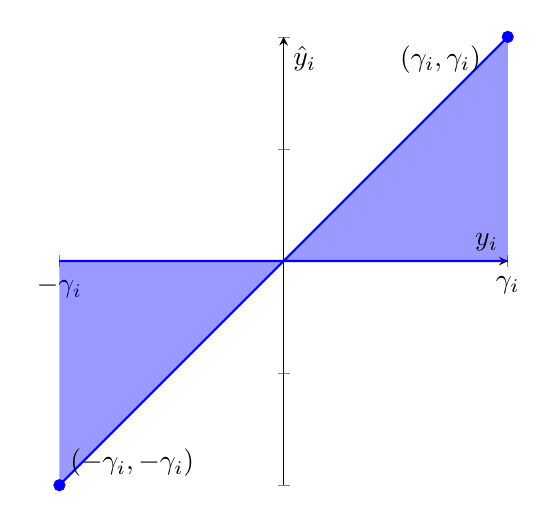
\begin{tikzpicture}
		\begin{axis}[
			xlabel={$y_i$},
			ylabel={$\hat{y}_i$},
			xmin=-2, xmax=2,
			ymin=-2, ymax=2,
			axis lines=center,
			samples=100, 
			unit vector ratio=1 1 1, scale=1, xtick   = {-2,2},
			xticklabels = {$-\gamma_i$,$\gamma_i$},
			yticklabels = {},
			]
			\addplot[blue, thick, fill=blue, fill opacity=0.4] {x} \closedcycle; 
			\addplot[blue, thick] {0}; 
			
			\addplot[only marks, mark=*, mark size=2pt, blue] coordinates {(-2,-2)};
			\node[label={above:$(-\gamma_i,-\gamma_i)$}] at (axis cs: -1.35, -2.1) {};
			
			\addplot[only marks, mark=*, mark size=2pt, blue] coordinates {(2,2)};
			\node[label={above:$(\gamma_i,\gamma_i)$}] at (axis cs: 1.4, 1.5) {};
		\end{axis}
	\end{tikzpicture}
\caption{The possible values of $\val(\hat{y}_i)=\ReLU(\val(x_i))-\ReLU(\val(x'_i))$ depending on $\val(y_i) = \val(x_i)-\val(x'_i)$.}
	\label{fig.1v}
\end{figure}


	
	Based on above constraints, we can sketch this simplified model:
	\begin{enumerate}
		\item For each input node, each output node, and each pre-activation and post-activation node in the hidden layers,  set one variable $y_i$. 
		\item Set constraints for input nodes.
		\item Set linear constraints . In this case, since the meaning of $y_i$ is $x_i-x'_i$, this constraints will not use the bias.
		\item Between pre- and post- activation nodes, set the MILP constraint described above.
	\end{enumerate}
	
	The key point is that, although this model sets 3 variables (and their binary variables) for each node in the network, only $y_i$  contributes to the final results, and we can ignore $x_i,x_i'$ (and their binary variables) during the optimization.
	
	As a result, we can relax the binary variables used to $\hat{x}_i = \ReLU(x_i)$ and $\hat{x}'_i = \ReLU(x'_i)$.
	
	Now the simplified model contains the same number of binary variables as the MILP model for local robustness. Hence this model runs much faster compared to the previous one. The trade-off is lower accuracy compared to the first model under unlimited time. In practice, with a reasonable timeout, this simplified model can usually obtain a better bound.
	
	One major disadvantage of this model is that the solution obtained through optimization may not be valid-i.e., the output computed by the network on the optimized inputs may not equal the output value in the solution. Nevertheless, it is meaningful to compute the upper bound. 
	
	%	However, in practice, with a reasonable timeout, this simplified model can usually obtain a better bound.
	%	
	\subsection{Improving the Accuracy of the Simplified Model}
	We can remove the disadvantage and improve the accuracy of the above simplified model by modifying the constraints, at the cost of increased computational time — a trade-off between accuracy and speed. 
	
	%	(This model has the same binary set, although the meaning of binary variable for $y_i$ is somehow different.)
	
	
	
	%	The exact constraints for $$ \begin{align*}
		%		&\hat{y}_i \geq -\hat{x}'_i \hspace*{1ex} \wedge \hspace*{1ex} \hat{y}_i \leq -\hat{x}'_i+a\beta_i  \hspace*{1ex}\wedge\hspace*{1ex} x_i'+y_i \leq a\beta_i \hspace*{1ex}\wedge\hspace*{1ex}  x_i'+y_i \geq (1-a)\alpha_i \\
		%		&\hat{y}_i \geq -\hat{x}'_i+(x_i'+y_i) \hspace*{1ex}\wedge\hspace*{1ex} \hat{y}_i \leq -\hat{x}'_i+(x_i'+y_i) +(a-1)\alpha_i \\
		%	\end{align*} 
	%	
	%	
	%	Moreover, we can add two more natural constraints: $x_i'+y_i \geq \alpha_i \hspace*{1ex}\wedge\hspace*{1ex}  x_i'+y_i \leq \beta_i.$
	
	
	
	
	
	\begin{figure}[t!]
		\centering
	\hspace*{-10ex}
	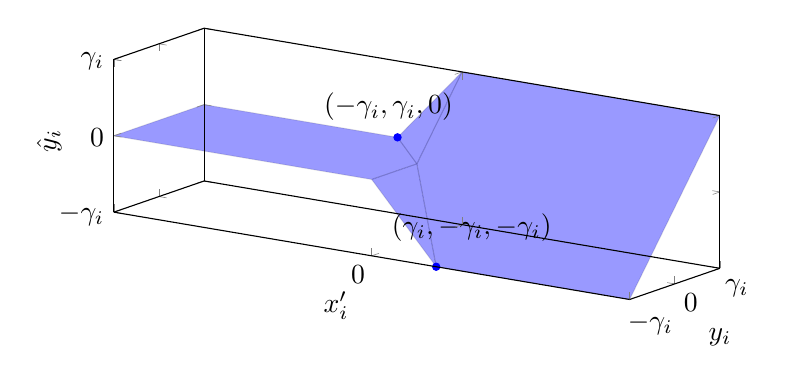
\begin{tikzpicture}[scale=0.65]
		\begin{axis}[	axis on top, xlabel = \(x'_i\),
			ylabel = {\(y_i\)}, zlabel = \(\hat{y}_i\),
			set layers=default,
			xmax = 4, xmin = -4,
			ymax = 1, ymin = -1,		
			zmax = 1, zmin = -1,
			unit vector ratio=1 1 1, scale=2.5,  ytick   = {-1,0,1},
			yticklabels = {$-\gamma_i$,$0$,$\gamma_i$}, xtick = {0},
			xticklabels = {$0$}, ztick   = {-1,0,1},
			zticklabels = {$-\gamma_i$,$0$,$\gamma_i$},
			view={35}{14},
			]
			\addplot3[ fill=blue,opacity=0.1, fill opacity=0.4] 
			coordinates {
				(0,0,0) (-1,1,0) (-4,1,0) (-4,-1,0) (0,-1,0) (0,0,0)
			};
			
			\addplot3[	fill=blue,opacity=0.1, fill opacity=0.4] 
			coordinates { (0,0,0) (0,1,1) (4, 1, 1) (4, -1, -1) (1,-1,-1) (0,0,0)
			};
			
			\addplot3[	fill=blue,opacity=0.1, fill opacity=0.4	] 
			coordinates { (0,0,0)  (-1,1,0) (0,1,1) (0,0,0)
			};
			
			\addplot3[	fill=blue,opacity=0.1, fill opacity=0.4	] 
			coordinates { (0,0,0)  (0,-1,0) (1,-1,-1) (0,0,0)
			};
			
			\addplot3[only marks, mark=*, mark size=2pt, blue] coordinates {(1,-1,-1)};
			\node[label={$(\gamma_i,-\gamma_i, -\gamma_i)$}] at (axis cs: 1.2, -0.5 ,-1) {};
			
			\addplot3[only marks, mark=*, mark size=2pt, blue] coordinates {(-1,1,0)};
			\node[label={$(-\gamma_i,\gamma_i, 0)$}] at (axis cs: -1, 0.8 ,0) {};			
			
		\end{axis}
	\end{tikzpicture}
	\caption{The outcome $\val(\hat{y}_i)=\ReLU(\val(x_i))-\ReLU(\val(x'_i))$ 
	depending on $\val(y_i) = \val(x_i)-\val(x'_i)$ and on $\val(x'_i)$.}
	\label{fig.2v}
\end{figure}
	
Given $\gamma_i$ as the upper bound of $y_i$, $\alpha_i,\beta_i$ be the upper and lower bound of $x_i,x_i'$, 
	the precise  constraints for $\hat{y}_i = \ReLU(x'_i+y_i)-\ReLU(x'_i)$ (along with $\hat{x}'_i=\ReLU(x'_i)$) are as follows:
	\begin{align*}
		& \begin{aligned}
			y_i + x'_i &\leq a\beta_i        &
			y_i &+ x'_i \geq (1-a)\alpha_i \\
			x'_i       &\leq a'\beta_i       & 
			x'_i       &\geq (1-a')\alpha_i \\
			\hat{y}_i  &\leq a\gamma_i       &
			\hat{y}_i  &\geq -a'\gamma_i \\
			\hat{y}_i  &\leq y_i + (1-a)\gamma_i  &
			\hat{y}_i  &\geq y_i - (1-a')\gamma_i \\
			\hat{y}_i  &\leq -x'_i + a\beta_i &
			\hat{y}_i  &\geq -x'_i + (1-a')\alpha_i \\
			\hat{y}_i  &\leq y_i + x'_i + (1-a)(-\alpha_i) &
			\hat{y}_i  &\geq y_i + x'_i + a'(-\beta_i)
		\end{aligned}
	\end{align*} Here, $a,a'$ are binary variables, and $a'$ is also the binary variable in the constraints for $\hat{x}'_i=\ReLU(x'_i)$. 
	

Similar to the second model, the constraints on $x_i$ for $\hat{x}_i=\ReLU(x_i)$ are not necessary, or at least can be relaxed without any loss in accuracy.
	
	%	\begin{align*}
		%		& y_i+x'_i \leq a\beta_i \quad\wedge \quad y_i+x'_i\geq (1-a)\alpha_i\\	
		%		& x_i' \leq a'\beta_i \quad\wedge \quad x_i'\geq (1-a')\alpha_i\\
		%		&\hat{y}_i \leq a\gamma_i \quad\wedge \quad	\hat{y}_i \geq -a'\gamma_i \\
		%		&	\hat{y}_i \leq y_i+(1-a)\gamma_i \quad\wedge \quad	\hat{y}_i \geq y_i - (1-a')\gamma_i \\
		%		&	\hat{y}_i \leq -x'_i+a\beta_i \quad\wedge \quad	\hat{y}_i \geq -x'_i+(1-a')\alpha_i \\
		%		&	\hat{y}_i \leq y_i+x'_i+(1-a)(-\alpha_i)\quad\wedge \quad	\hat{y}_i \geq y_i+x'_i+a'(-\beta_i) \\
		%	\end{align*} 
	
	The following plot illustrates the constraints described above.
	

	In practice, when we relax the constraints for a node, we will convert $a_i$ and $a_i'$ to continuous variables together. In principle, we can also choose to change  only one of those two binary variables.
	
	%	The relaxation of this model is similar: let $a$s and $a'$s be continuous variables instead of binary/integer variables. Unlike the first model in this section, relaxing a few nodes does not lose too much accuracy.
	
	A special relaxation approach of this model is to treat the binary variables $a'$ appearing in the above constraints and the binary variables for $\hat{x}'_i=\ReLU(x'_i)$ as distinct variables, and relax only the latter. 
	
	This approach has a similar disadvantage as the model in the previous section: the output computed by the network on the optimized inputs may not equal the output value in the solution. Similarly, it is meaningful to compute the upper bound using this approach. 
	
	
	


	\section{Experimental Evaluation}
	
	We implemented our code in Python 3.8.
	Gurobi 9.52 was used for solving LP and MILP problems. We conducted our evaluation on an AMD Threadripper 7970X  ($32$ cores$@4.0$GHz) with 256 GB of main memory and 2 NVIDIA RTX 4090. 
	
	We will do experiments on two networks for MNIST dataset and another physical model. Two MNIST have the same structure. They are full-connected DNN with 5, 10 outputs and 784 inputs; each hidden layer has 100 neurons. One of them is a normally trained neural network and another is for trained for adversarial robustness. We call them MNIST $5\times100$-Normal and MNIST $5\times 100$-DiffAI. As the name shows MNIST $5\times 100$-DiffAI has a better robustness. The physical network is a simplified model with 10 input neurons, 26 output neurons, and 2 hidden layers with 50 neurons each.
	
	\subsection{Experiment results for robustness (MNIST)}
	

	
	\begin{table}[h!]
	\begin{tabular}{|l|c|c|c|c|}\hline\hline
		$L_1\leq 0.5$ &        Bound $\downarrow$ &  Sol. &      Worst-Case $\uparrow$ &  Time \\\hline \hline
		1v, $375 \times 1$ & 17.4724 & 0.9089  ?? & 0.0917 & 43200s \\\hline 
		2v, $375 \times 2$ & 21.0135 & 8.4672& 0.2229 & 43200s \\\hline		
		2v, $450 \times 2$ & 12.0097 & 3.4408 & {\bf 0.2584} & 43200s \\\hline
		1v, $500 \times 1$ & ?? & ?? & ?? & 43200s \\\hline 
		3v, $500 \times 3$ & ?? & ?? & ?? & 43200s \\\hline 
	 2v, $500 \times 2$ & {\bf 8.7608} & nan & nan & 43200s \\\hline\hline

	 2v, $485 \times 2$ & 20.6460 & 1.9152 & {\bf 0.3722} & 130000s \\\hline\hline

		 2v, $500 \times 2$ & {\bf 8.2573} & nan & nan & 260000s \\\hline\hline
		 
	\end{tabular}
	\caption{Comparison of "1v", "3v" and "2v" models 
	to obtain bounds on $\beta^{0.5}_{0,1}$ on the {\bf full dimension} MNIST DNN, for timeouts of 43200s, 130000s and 260000s, where 375, 450, 485 or 500 ($\times 1$, $\times 2$, $\times 3$) neurons use binary variables.}
\end{table}

On the full space, we reach bounds of $8.2$ (on $\beta^{.5}_{0,1}$), which is too pessimistic as it allows to certify 0 image robust. The worst-case found by the "2v" $485 \times 2$ binary variables after 130000s only displays a difference of 
$0.37$, $20 \times$ away from the bound found.

\begin{figure*}[t!]
	\centering
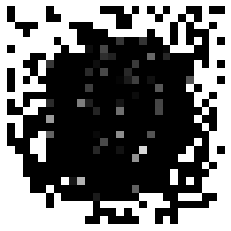
\includegraphics[scale=0.5]{image.png} \hspace{0.8cm}
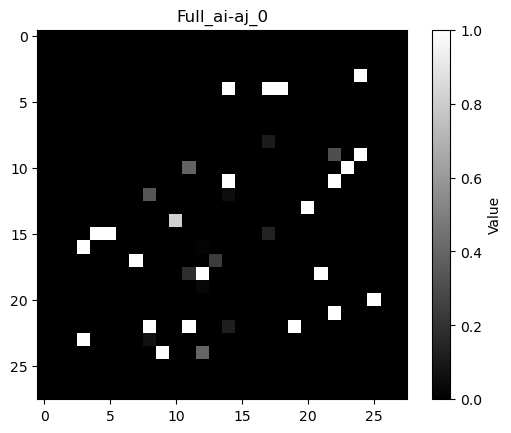
\includegraphics[scale=0.5]{perturb.png}
\caption{An improbable image and its perturbation (difference around x=11, y=18) 
with maximal $\beta^{.5}_{0,1}=0.37$ for MNIST as obtained by the "2v" $485 \times 2$ model in full 758 dimension image space.}
\end{figure*}	




\paragraph{Reduced space}

We now consider a PCA model order reduction to avoid considering improbable images, 
speed up obtaining the bounds, and obtain less pessimistic bounds.
We settle on 20 orders, as the MNIST DNN considered run on a images obtained from projecting to the reduced order and projected back to the full dimension 
display the same accuracy of $97$\% as the DNN on the original images, meaning no accuracy is lost from reducing to 20 dimensions, which is the only thing which matters. On such a reduced space, bounds obtained are much more precise, and one can certify robustness of images online.



	\begin{table}[h!]
	\begin{tabular}{|l|c|c|c|c|}\hline\hline
		$L_1\leq 0.5$ &        Bound $\downarrow$ &  Sol. &      Worst-Case $\uparrow$ &  Time \\\hline \hline
		
1v, $?? \times 1$ & ?? & ?? & ?? & ?? \\\hline 
		3v, $?? \times 3$ & ?? & ?? & ?? & ?? \\\hline 
	 2v, $?? \times 2$ & ?? & ?? & ?? & ?? \\\hline\hline
	 
		1v, $?? \times 1$ & ?? & ?? & ?? & ?? \\\hline 
		3v, $?? \times 3$ & ?? & ?? & ?? & ?? \\\hline 
	 2v, $?? \times 2$ & ?? & ?? & ?? & ?? \\\hline\hline
	 
	\end{tabular}
	\caption{Comparison of "1v", "3v" and "2v" models 
	to obtain bounds on $\beta^{0.5}_{0,1}$ on the {\bf 20 dimension}  reduced order MNIST DNN, for timeouts of ??s, and ??s , where ??,  or 500 ($\times 1$, $\times 2$, $\times 3$) neurons use binary variables.}
\end{table}






\begin{figure*}[t!]
	\centering
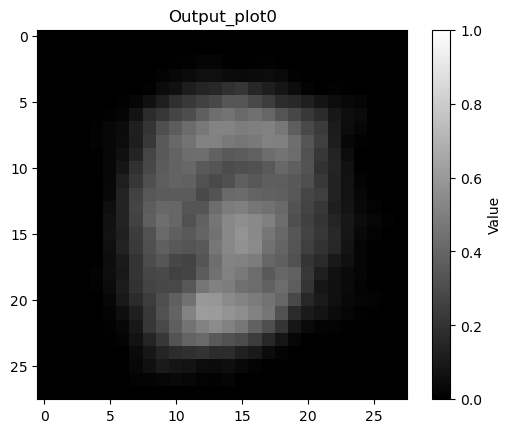
\includegraphics[scale=0.5]{redimage.png} \hspace{0.8cm}

\includegraphics[scale=0.5]{redperturb.png}
\caption{An image and its perturbation from the 20-dimension reduced space with maximal $\beta^{.5}_{0,1}=0.17$ for MNIST as obtained by the "2v" $500 \times 2$ model.}
\end{figure*}	

	
	
\begin{table}[h!]
	\begin{tabular}{|l|c|c|c|c|}\hline\hline
		model &    $L_1\leq 0.5$ & $L_1\leq 1$ & $L_1\leq 1.5$ &  $L_1\leq 2$ \\\hline \hline
		1v, $? \times 1$ & $80 \%$ & $32\%$ & $7\%$ & $0\%$ \\\hline
		3v, $? \times 3$ & {\bf 86 \%} & {\bf 53\%} & {\bf 20\%} & {\bf 4\%} \\\hline
		2v, $? \times 2$ & ?? & ?? & ?? & ?? \\\hline \hline
	\end{tabular}
	\caption{Comparison of "1v", "3v" and "2v" models 
	in the percentage of images they can certify in real-time for different values of $L_1$ perturbations.}
\end{table}


	


\subsection{Experiment results for regression (Pipe strain)}
	
	For the pipe system, to find a example of large difference on outputs is one of the main aims.

	\begin{figure*}[t!]
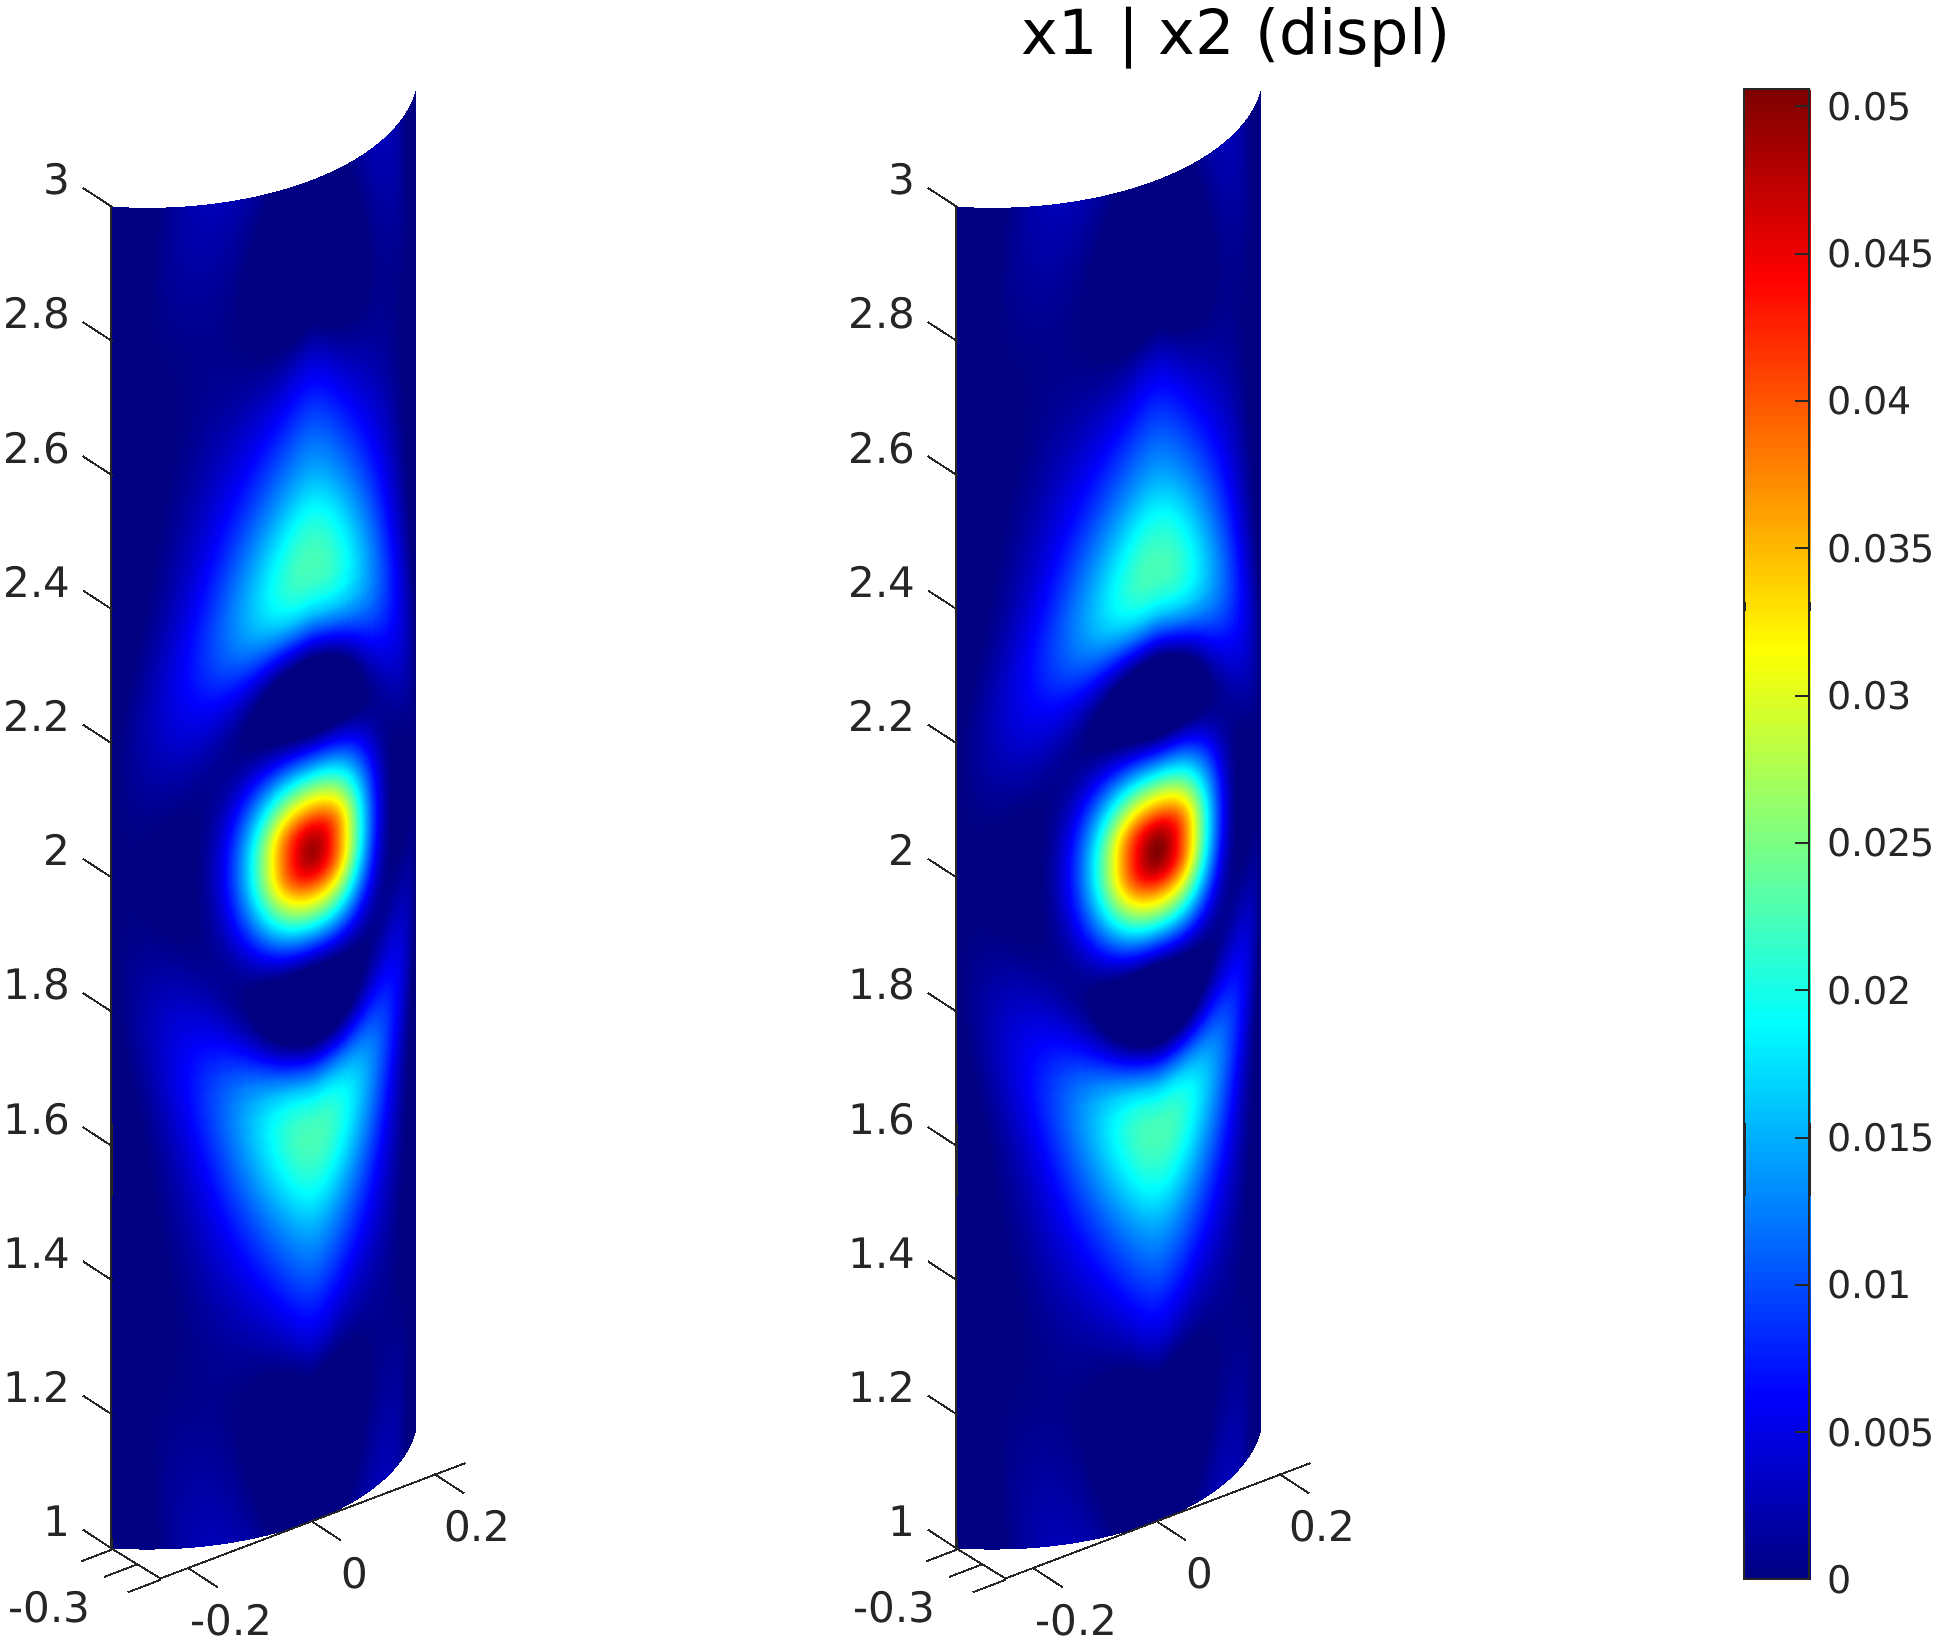
\includegraphics[scale=0.5]{deform.png} \hspace{0.8cm}
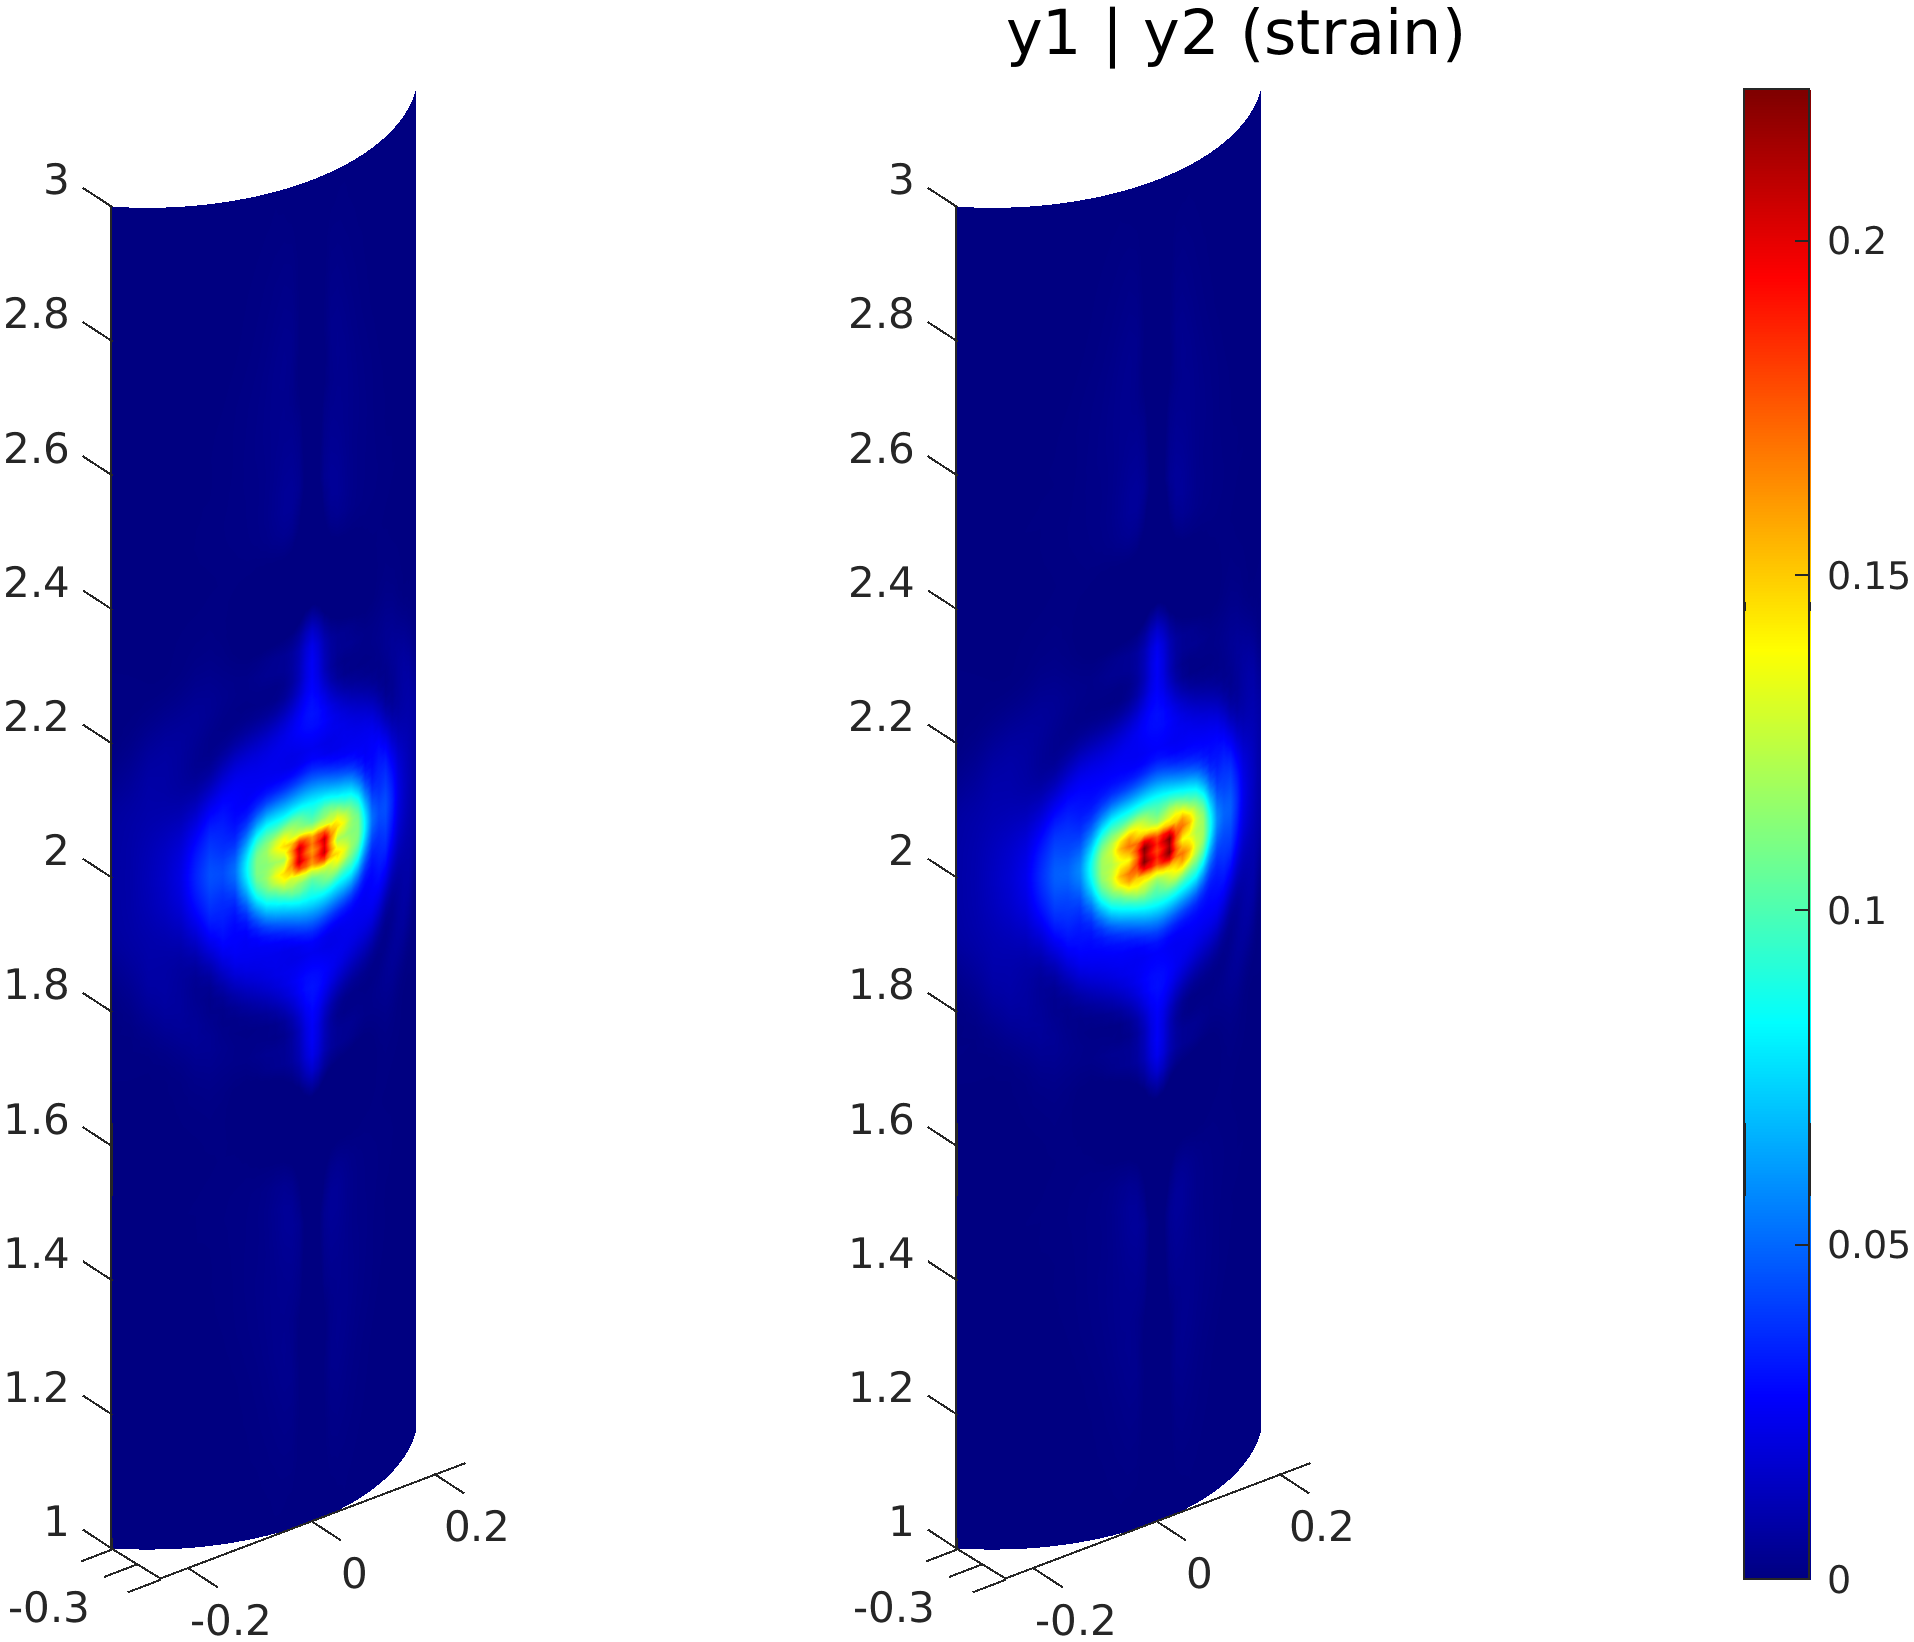
\includegraphics[scale=0.5]{strain.png}
\caption{2 slightly different deformations and their associated quite different strain as obtained by the "2v" $100 \times 2$ model.}
\end{figure*}	


	The network of Pipe system is relatively simple and in the tests, we will open all $\ReLU$ nodes.

	

	We will compare the results of different modeling methods.
	
	\vspace*{1ex}
	
	\iffalse
	\begin{table}[h!]
	\begin{tabular}{|l|l|l|l|l|}\hline
		$L_1\leq 0.83$ &        Bound $\downarrow$ &  Solution $\uparrow$ &      Real $\uparrow$ &  Time \\\hline
		1v,open 100 &     {\bf 0.035613} &  0.035613 &                       0.01288 & 10608 \\\hline
		3v,open 100 &     0.040074 &  0.028934 &                      0.021441 & 10922 \\\hline
		%3v,open 100 &     0.039824 &  0.028832 &                      0.022255 & 22153 \\\hline
		2v,open 100 &     0.046719 &  0.024364 &  {\bf 0.024436} & 10922 \\\hline
	\end{tabular}
	\caption{Comparison of 1v,2v and 3v models on the pipe system with a fixed timeout of 10.000s.}
\end{table}
\fi
	
		
	\begin{table}[h!]
	\begin{tabular}{|l|c|c|c|c|}\hline\hline
		$L_1\leq 0.83$ &        Bound $\downarrow$ &  Sol. &      Worst-Case $\uparrow$ &  Time \\\hline \hline
		1v, $100 \times 1$ &     {\bf 0.0356} &  $0.0356$ & $0.0191$ &   1000s \\\hline
		3v, $100 \times 3$&     0.0414 &  0.0254 &  0.0166 &  1000s \\\hline
		2v, $100 \times 2$&     0.0418 &  0.0229 &   {\bf 0.0229} &  1000s \\\hline \hline
		3v, $90 \times 3$&      ?? &  ?? &  ?? & 14523s \\\hline
		3v, $100 \times 3$&      {\bf 0.0350} &  0.0272 &  0.0216 & 14523s \\\hline
		2v, $90 \times 2$&     ?? &  ?? &   ?? & 14523s \\\hline
		2v, $100 \times 2$&     0.0360 &  0.0236 &    {\bf 0.0236} & 14523s \\\hline \hline
		3v, $100 \times 3$&     {\bf 0.0329} &  0.0277 &  0.0165 & 72126s \\\hline
		2v, $100 \times 2$&     0.03375 &  0.0244 &  {\bf 0.0245} & 72126s \\\hline\hline
	\end{tabular}
	\caption{Comparison of "1v", "3v" and "2v" models on the pipe system with a fixed timeout of 1000s, 14523s and 72126s, where 90 ($\times 2$, $\times 3$) or all 100 ($\times 1, \times 2,\times 3$) neurons use binary variables.
	L1 corresponds to $3.9$ or $4$, and results should be the sum of 10 pixels, so around 10 times higher values.}
\end{table}

	
	
	
	
	
	 
	
	
	\newpage

	\hfill

	\newpage
	
	
	\bibliography{references}
	
	
\end{document}
